\pdfoutput=1
\documentclass[11pt]{article}
\usepackage[margin=1in]{geometry}
\usepackage{amsmath,amssymb,amsthm,booktabs,array}
\usepackage[shortlabels]{enumitem}
\usepackage[hidelinks]{hyperref}
\usepackage{algorithm}
\usepackage[noend]{algpseudocode}
\usepackage{tikz}
\usetikzlibrary{arrows.meta,backgrounds,calc,positioning,fit}
\tikzset{
  v/.style={circle,draw,fill=white,inner sep=0pt,minimum size=6pt,line width=0.6pt},
  d/.style={circle,fill=black,inner sep=0pt,minimum size=4.5pt},
  e/.style={line width=0.6pt},
  faint/.style={line width=0.5pt,black!30},
  arc/.style={line width=0.6pt,-{Stealth[length=4.5pt]}},
  lab/.style={font=\scriptsize},
  box/.style={draw,rounded corners=2pt,line width=0.6pt,align=center,font=\footnotesize,inner sep=4pt,minimum height=20pt},
  tool/.style={box,fill=black!6},
  main/.style={box,line width=1.1pt},
}


\setlist{itemsep=1pt,topsep=3pt}

\newtheorem{theorem}{Theorem}[section]
\newtheorem{lemma}[theorem]{Lemma}
\newtheorem{corollary}[theorem]{Corollary}
\newtheorem{fact}[theorem]{Fact}
\theoremstyle{definition}
\newtheorem{definition}[theorem]{Definition}
\theoremstyle{remark}
\newtheorem{remark}[theorem]{Remark}

% statements with names
\theoremstyle{plain}
\newtheorem*{namedinner}{\namedtext}
\newenvironment{named}[1]{\def\namedtext{#1}\phantomsection\namedinner}{\endnamedinner}

\newcommand{\ThmBip}{\hyperref[thm:bip]{Bipartite Matching Theorem}}
\newcommand{\ThmWeight}{\hyperref[thm:weight]{Weighted Matching Theorem}}
\newcommand{\ThmGen}{\hyperref[thm:gen]{General Matching Theorem}}
\newcommand{\ThmCert}{\hyperref[thm:cert]{Certificate Theorem}}
\newcommand{\ThmTw}{\hyperref[thm:tw]{Treewidth Theorem}}
\newcommand{\LemPath}{\hyperref[lem:path]{Path Lemma}}
\newcommand{\LemMS}{\hyperref[lem:ms]{Multi-Source Lemma}}
\newcommand{\LemLabels}{\hyperref[lem:labels]{Exact Labels Lemma}}
\newcommand{\ThmOff}{\hyperref[thm:off]{Offset Theorem}}
\newcommand{\LemLA}{\hyperref[lem:la]{Linear Algebra Lemma}}
\newcommand{\AlgPath}{\textsc{SimplePath}}
\newcommand{\AlgBip}{\textsc{InsertHub}}
\newcommand{\AlgWeight}{\textsc{WeightedInsertHub}}
\newcommand{\AlgElim}{\textsc{BagElimination}}
\newcommand{\AlgMates}{\textsc{FindMates}}

\newcommand{\Ot}{\tilde O}
\newcommand{\dist}{\mathrm{dist}}
\newcommand{\sep}{\mathrm{sep}}
\newcommand{\Int}{\mathrm{Int}}
\newcommand{\In}{\mathrm{In}}
\newcommand{\Out}{\mathrm{Out}}
\newcommand{\rank}{\operatorname{rank}}
\newcommand{\odd}{\mathrm{odd}}
\newcommand{\reach}{\rightsquigarrow}
\newcommand{\F}{\mathbb{F}}

\title{Exact Maximum Matching in Planar Networks\\ in the CONGEST Model}
\hypersetup{pdftitle={Exact Maximum Matching in Planar Networks in the CONGEST Model},pdfauthor={Sebastian Senge}}
\author{Sebastian Senge\\ Independent Researcher}
\date{}

\begin{document}
\maketitle

\begin{abstract}
We give exact algorithms for maximum matching in the CONGEST model on planar networks. Their round
bounds depend on the hop diameter $D$ and only polylogarithmically on the number of vertices, and
$\Omega(D)$ rounds are necessary. Previous exact bounds depend on the size $s^*$ of a maximum matching, as
$\Ot(s^*)$ rounds, or on the treewidth $\tau$, as $\Ot(\tau^4D+\tau^7)$ rounds for bipartite networks. On bipartite planar
networks, the classical separator scheme with one exact shortest-path computation per inserted vertex gives
$\Ot(D^3)$ rounds. Our results are these:
\begin{itemize}[leftmargin=1.5em]
\item Bipartite planar networks: a maximum matching in $\Ot(D^2)$ rounds, deterministic once the decomposition is given.
\item Bipartite planar networks with integer weights: a maximum weight matching and an optimal dual in $\Ot(D^3)$ rounds, with a complete proof of the exact distance labels behind that bound.
\item General planar networks: a maximum matching in $\Ot(D^2)$ rounds with high probability, and with no error once the decomposition is given, together with the set of vertices that some maximum matching misses, their neighbours and the remaining vertices.
\item Networks of treewidth $\tau$, not necessarily planar or bipartite: a maximum matching in $\Ot(\tau^3D+\tau^5)$ rounds with high probability.
\item Two tools on planar digraphs: a simple directed path between two given vertices in $\Ot(D)$ rounds, and exact distance labels in $\Ot(D^2)$ rounds.
\end{itemize}
Minimum vertex cover, maximum independent set and vertex-disjoint paths follow. The bipartite algorithms insert
separator vertices one at a time, each along one simple path. The general algorithm eliminates a random
alternating matrix along the tree of a recursive decomposition. On bipartite planar networks the exponent of $D$ falls from $3$ to $2$. For general planar networks we know of no
earlier exact bound polynomial in $D$ alone, and the new bound is below $s^*$ when $D$ is well below $\sqrt{s^*}$. The combinatorial core of
the path algorithm, of the dual update and of the matrix steps is machine-checked in Lean~4 with Mathlib. The
CONGEST algorithms, their round counts and all other arguments are proved on paper only, and numerical
checks support them without being used in any proof.
\end{abstract}

\section{Introduction}

\subsection{Matching in the CONGEST model}

In the CONGEST model the input graph is the network itself. Every vertex is a processor that
initially knows its incident edges. Computation proceeds in synchronous rounds, in every round each
vertex can send a message of $O(\log n)$ bits over each incident edge, and local computation is free.
The complexity of an algorithm is its number of rounds, as a function of the number $n$ of vertices
and of the hop diameter $D$. A \emph{matching} is a set of edges in which no two share a vertex, and
at the end every vertex has to know its partner in a matching of maximum size, or of maximum
weight in the weighted version.

Exact maximum matching in general networks takes $\Ot(s^*)$ rounds~\cite{IKY23}, randomized, where
$s^*$ is the size of a maximum matching, and it took $\Ot(s^{*3/2})$ rounds before~\cite{KI21}. In
bipartite networks, $O(s^*\log s^*)$ rounds were shown in~\cite{AKO18}. These bounds can be close to
$n$ even when $D$ is small. On networks of treewidth $\tau$, a maximum matching of a bipartite network
takes $\Ot(\tau^4D+\tau^7)$ rounds~\cite[Theorem~4]{IKNS22}. A planar network of hop diameter $D$
has treewidth $O(D)$, so this gives $\Ot(D^7)$ rounds. It was also observed in~\cite{IKNS22} that the
idea behind that bound does not carry over to general graphs, since a shortest $2$-coloured walk need
not be simple.

Planar networks have seen progress on other problems through the bounded diameter decomposition
of~\cite{LP19}: exact reachability in $\Ot(D)$ rounds~\cite{P20}, and exact shortest paths and
maximum flow in $\Ot(D^2)$ rounds~\cite{LP19,P20,ADPW25}. Exact minimum cost flow on planar graphs
takes $n^{1/2+o(1)}D$ rounds~\cite{dV23}, for one $st$-flow on the communication graph. Matching
needs a super-source and a super-sink, and these can break planarity: on the cube every face holds
two of the four vertices of one side, so even one apex on that side gives a non-planar graph. So the planar bound of~\cite{dV23} does not give matching by its statement. Approximate shortest paths on
planar digraphs take $\Ot(D/\varepsilon)$ rounds by~\cite{LTY26}. That proof reads distances from labels and gives no
path, so it does not give the \LemPath{}.

Further bounds follow from these tools, although we did not find them stated. The scheme of~\cite{LT80} inserts the
vertices of a separator one at a time. With one exact SSSP of~\cite[Lemma 4]{P20} per insertion, it gives a maximum
bipartite matching, also with weights, in $\Ot(D^3)$ rounds. A perfect matching of a bipartite planar network, or the
report that none exists, takes $\Ot(D^2)$ rounds with high probability through the dual distances of~\cite{ADPW25} and the
demand routing of~\cite{MN95}. Maximum matching does not follow from that route, since free vertices would need a
super-source, which is not planar. To our knowledge there is no earlier exact bound for general planar networks that is polynomial in $D$ alone.

A lower bound of $\Omega(D)$ holds for maximum matching, already on paths. Take a path with an even number of vertices and
shift it by one vertex. A vertex in the middle sees the same neighbourhood in both for about $D/2$ rounds, while its partner
in the unique perfect matching differs. The gap between $\Ot(D^2)$ and $\Omega(D)$ stays open.

\subsection{Results}

Table~\ref{tab:results} compares the bounds. The statements follow. Throughout, $G$ is a connected
network with $n$ vertices and hop diameter $D$, planar unless stated otherwise, and $\Ot$ hides
factors polylogarithmic in $n$. All planar algorithms first compute the decomposition of Section~\ref{sec:bdd}, whose
construction in~\cite{LP19} is randomized. So determinism and zero error below are meant given a decomposition with
the stated properties.

\begin{table}[t]
\centering\small
\begin{tabular}{@{}p{5.5cm}lp{6.2cm}@{}}
\toprule
Problem & This paper & Previous best bound\\
\midrule
Maximum matching, bipartite planar & $\Ot(D^2)$ & $\Ot(D^3)$, implied by~\cite{LT80,P20}; $\Ot(D^7)$, implied by~\cite{IKNS22}; $O(s^*\log s^*)$~\cite{AKO18}\\
Maximum weight matching, bipartite planar & $\Ot(D^3)$ & $\Ot(D^3)$, implied by~\cite{LT80,P20}, with its proof deferred\\
Minimum vertex cover, bipartite planar & $\Ot(D^2)$ & $\Ot(D^3)$, implied by~\cite{LT80,P20}\\
Maximum matching, general planar, zero error & $\Ot(D^2)$ & $\Ot(s^*)$~\cite{IKY23}\\
Maximum matching, treewidth $\tau$ & $\Ot(\tau^3D+\tau^5)$ & $\Ot(\tau^4D+\tau^7)$, bipartite only~\cite{IKNS22}\\
Simple directed $st$-path, planar & $\Ot(D)$ & $\Ot(D^2)$, from exact directed SSSP~\cite{P20}\\
\bottomrule
\end{tabular}
\caption{Bounds for exact problems. Previous bounds are results of other authors or direct consequences of them,
to our knowledge. ``Implied'' means that the bound is not stated there: $\Ot(D^7)$ follows from the
treewidth bound, since a planar network has treewidth $O(D)$, and $\Ot(D^3)$ from the scheme of~\cite{LT80} with one
exact SSSP per insertion. The algorithms for general planar networks and for treewidth $\tau$, and the one
of~\cite{IKY23}, use randomness beyond the decomposition.}
\label{tab:results}
\end{table}

\begin{named}{Path Lemma}\label{lem:path}
Let $G$ be a planar digraph whose underlying graph has hop diameter $D$, and let $s,t$ be vertices
with a directed $st$-path. In $\Ot(D)$ rounds every vertex learns its arcs on one simple directed
$st$-path. The algorithm is deterministic relative to the decomposition.
\end{named}

\begin{named}{Bipartite Matching Theorem}\label{thm:bip}
A maximum matching of a bipartite planar network is computed in $\Ot(D^2)$ rounds, deterministically
relative to the decomposition.
\end{named}

\begin{named}{Weighted Matching Theorem}\label{thm:weight}
A maximum weight matching of a bipartite planar network with integer weights in $\{0,\dots,n^{O(1)}\}$,
together with an optimal integer dual, is computed in $\Ot(D^3)$ rounds. A minimum weight perfect
matching, or the report that none exists, takes the same bound.
\end{named}

\begin{named}{Multi-Source Lemma}\label{lem:ms}
For any set $S$ of sources in a planar digraph, every vertex learns in $\Ot(D)$ rounds whether some
source reaches it.
\end{named}

\begin{corollary}\label{cor:konig}
A minimum vertex cover and a maximum independent set of a bipartite planar network take $\Ot(D^2)$
rounds.
\end{corollary}

\begin{named}{General Matching Theorem}\label{thm:gen}
In $\Ot(D^2)$ rounds every vertex of a planar network learns its mate in a matching $M$. Always $M$ is a
matching, and it is maximum with probability at least $1-n/p$ for a prime $p=n^{O(1)}$ that the
algorithm chooses.
\end{named}

\begin{named}{Certificate Theorem}\label{thm:cert}
Let $D(G)$ be the set of vertices that some maximum matching misses, $A(G)$ the set of their neighbours
outside $D(G)$, and $C(G)$ the set of remaining vertices. These are the \emph{canonical sets} of $G$, whose
structure is described in~\cite{LoP86}. In a further $\Ot(D^2)$ rounds every vertex learns its label in sets
$D',A',C'$, and the network checks with no error whether $M$ is maximum and $D'=D(G)$, $A'=A(G)$, $C'=C(G)$.
The check passes with probability at least $1-O(1/n)$. So maximum matching and the canonical sets have a
zero-error algorithm with $\Ot(D^2)$ rounds with high probability: on a failed
check it starts again with new randomness.
\end{named}

\begin{named}{Treewidth Theorem}\label{thm:tw}
Let $G$ be a network of treewidth $\tau$, not necessarily planar. With high probability, in
$\Ot(\tau^3D+\tau^5)$ rounds every vertex learns its mate in a maximum matching of $G$ and its
canonical set.
\end{named}

\begin{corollary}\label{cor:paths}
In the bounds of the \ThmCert{} and the \ThmTw{}: a minimum vertex cover and a maximum independent set
of a bipartite network, and for a digraph with vertices $s,t$ the maximum number $\kappa$ of paths from
$s$ to $t$ that are vertex disjoint except at $s,t$, with $\kappa$ such paths, and a minimum set of
vertices that separates $s$ from $t$ if there is no arc from $s$ to $t$.
\end{corollary}

We also give two tools of independent use. The \LemLabels{} and the \ThmOff{} in
Section~\ref{sec:weighted} compute exact distance labels of a planar digraph in $\Ot(D^2)$ rounds and
answer queries from a virtual source with arbitrary offsets. The \LemLA{} in Section~\ref{sec:general}
computes the rank of a symmetric or alternating matrix with entries on the edges of $G$, and solves
linear systems in it.

The bound $\Ot(D^2)$ improves on $\Ot(s^*)$ only if $D$ is below about $\sqrt{s^*}$. On a square grid
the two agree, and on planar networks with small diameter, such as those with a few vertices of large degree, the
difference can be large.

\begin{remark}[conditional bounds]\label{rem:cond}
A companion work~\cite{S26} computes exact SSSP in $\Ot(D)$ rounds given a hypothesis on approximate
distance labels, the Label Hypothesis stated there. Given this hypothesis, the \ThmWeight{} holds in
$\Ot(D^2)$ rounds, since each insertion below uses one SSSP. A perfect matching of a bipartite planar
network, or the report that none exists, takes $\Ot(D)$ rounds with high probability given the hypothesis, by the
reduction for negative weights of~\cite{FHLRS25} with the demand routing of~\cite{MN95}; this is claimed in the
repository of~\cite{S26} and not in this paper. Maximum matching does not follow from it, since free vertices would need a
super-source, which is not planar.
\end{remark}

\subsection{How the algorithms fit together}

Figure~\ref{fig:overview} shows the structure. All algorithms use the same recursive decomposition:
bags of hop diameter $\Ot(D)$, split along separators of $\Ot(D)$ vertices, in a tree of height
$O(\log n)$. Bags of one depth share each edge at most twice, so they run in parallel.

\begin{figure}[t]
\centering
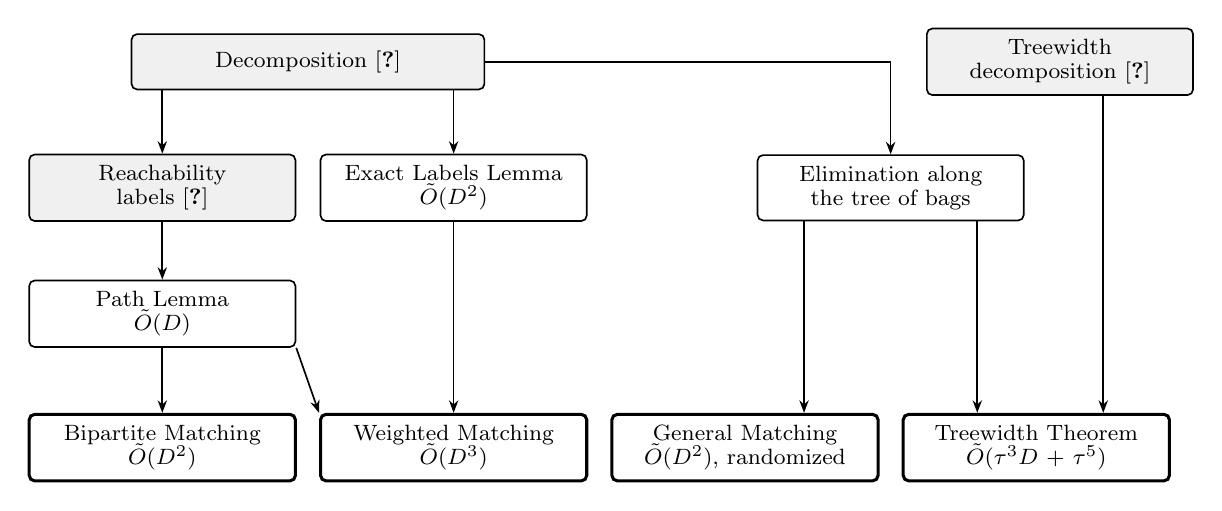
\begin{tikzpicture}[x=1cm,y=1cm]
\tikzset{every node/.append style={text width=3.1cm}}
\node[tool,text width=4.2cm] (bdd) at (-3.7,3.5) {Decomposition~\cite{LP19}};
\node[tool] (tw) at (5.85,3.5) {Treewidth\\[-1pt]decomposition~\cite{IKNS22}};
\node[tool] (lab) at (-5.55,1.9) {Reachability\\[-1pt]labels~\cite{P20}};
\node[box] (el) at (-1.85,1.9) {Exact Labels Lemma\\[-1pt]$\tilde O(D^2)$};
\node[box] (te) at (3.7,1.9) {Elimination along\\[-1pt]the tree of bags};
\node[box] (path) at (-5.55,0.3) {Path Lemma\\[-1pt]$\tilde O(D)$};
\node[main] (bip) at (-5.55,-1.4) {Bipartite Matching\\[-1pt]$\tilde O(D^2)$};
\node[main] (wei) at (-1.85,-1.4) {Weighted Matching\\[-1pt]$\tilde O(D^3)$};
\node[main] (gen) at (1.85,-1.4) {General Matching\\[-1pt]$\tilde O(D^2)$, randomized};
\node[main] (trw) at (5.55,-1.4) {Treewidth Theorem\\[-1pt]$\tilde O(\tau^3D+\tau^5)$};
\draw[arc] (bdd.south -| lab) -- (lab);
\draw[arc] (bdd.south -| el) -- (el);
\draw[arc] (bdd.east) -| (te.north);
\draw[arc] (lab) -- (path);
\draw[arc] (path) -- (bip);
\draw[arc] (path.south east) -- (wei.north west);
\draw[arc] (el) -- (wei);
\draw[arc] (te.south -| 2.6,0) -- (gen.north -| 2.6,0);
\draw[arc] (te.south -| 4.8,0) -- (trw.north -| 4.8,0);
\draw[arc] (tw.south -| 6.4,0) -- (trw.north -| 6.4,0);
\end{tikzpicture}

\caption{How the results depend on each other. Shaded boxes are published tools, used as black boxes, and
boxes with thick borders are the main theorems.}
\label{fig:overview}
\end{figure}

\paragraph{Bipartite networks.} The classical scheme of~\cite{LT80} solves the pieces of a separator
and then inserts the separator vertices one at a time. Each insertion changes the matching along at
most one augmenting path. There are $\Ot(D)$ insertions per depth. One exact SSSP per insertion gives $\Ot(D^3)$ in all, so for
$\Ot(D^2)$ we need an augmenting path in $\Ot(D)$ rounds. Reachability in this time is known from~\cite{P20}, but a path is not: the flip needs a
\emph{simple} path. Our algorithm \AlgPath{} assigns requests top down. Every vertex computes them
for all its bags with no communication, from labels broadcast once. Paths are then realized bottom up,
with a loop erasure that only has to run on separators and needs $\Ot(D)$ words per bag.

\paragraph{Weights.} The insertion becomes a primal-dual step with one exact shortest-path
computation per insertion. For digraphs, the bound $\Ot(D^2+D|S|)$ for a set $S$ of sources is stated in~\cite[Lemma 4]{P20}, with the proof deferred
to a full version. We prove the \LemLabels{}, a bottom-up computation with $\Ot(D^2)$ words per bag. Used with the Virtual
Source Lemma of~\cite{S26}, it allows any offsets at no extra cost.

\paragraph{General networks.} Augmenting paths in the residual digraph do not work without
bipartiteness, and we use algebra as in the sequential work of~\cite{MS06,FLPSW18}. \AlgElim{} eliminates a random alternating
matrix along the tree of bags. A singular interior block is handled by keeping at most as many further
indices as the boundary has, so each bag moves $\Ot(D^2)$ words. \AlgMates{} then finds mates top
down, with two solves per hub. Since a bag holds a factorization, one solve takes $\Ot(D)$ rounds. The check of the \ThmCert{} runs in the bags and
removes all error from the output.

\subsection{Verification}

The theorems are proved on paper. The black boxes of~\cite{LP19,P20,IKNS22} were read and not proved
again, and the proofs of~\cite[Lemmas 10 to 13]{P20} are not in the conference text. The Lean
formalization covers the combinatorial core, listed exactly in Section~\ref{sec:lean}: loop erasure, disjointness of intervals,
the
query fact and a form of the cutting fact, the dual update and the flip, and the matrix identities of the elimination. It does not cover planarity,
the decomposition, knowledge of the vertices or any round count.

There is no simulation of CONGEST. The scripts of Section~\ref{sec:numerics} run the logic centrally
on instances checked for planarity, against independent solvers, with negative controls. They check
words per bag, not rounds. 

\section{Preliminaries}\label{sec:prelim}

\subsection{Decompositions}\label{sec:bdd}

Words have $O(\log n)$ bits. A planar embedding can be computed in $\Ot(D)$ rounds~\cite{GH16}. We use
the \emph{bounded diameter decomposition} (BDD) of~\cite{LP19} in the form of~\cite{P20}, computed
in $\Ot(D)$ rounds. It is a tree of \emph{bags} of height $O(\log n)$, whose root is $G$, and in which
every child is a subgraph of its parent. Each bag $Y$ has a separator $\sep(Y)$, with the following
properties.
\begin{enumerate}[(B1)]
\item Every bag has hop diameter $O(D\log n)$, and $|\sep(Y)|=O(D\log n)$.
\item Every edge of a bag that is not a leaf lies in a child of the bag, and every edge lies in at most two bags per level.
\item A vertex of $\sep(Y)$ lies on at most three children of $Y$. Any other vertex of $Y$ lies on exactly one.
\item A leaf has $O(D\log n)$ vertices and $\sep(Y)=V(Y)$.
\end{enumerate}
The separator used in~\cite{LP19} is randomized. Deterministic planar separators in $\Ot(D)$ rounds are given
in~\cite{JMR25,ADW26a}, where it is stated that they derandomize planar algorithms whose only randomized part is the separator. We
did not check the construction of the decomposition for this. We call an algorithm \emph{deterministic relative to the
decomposition} if it is deterministic once a BDD with (B1) to (B4) is given, and zero error has the same meaning.

Bags of one level run in parallel by (B2), at a cost of a factor $2$. A BFS tree $T_Y$ of each bag
costs $\Ot(D)$ rounds once. A broadcast or convergecast of $w$ words over $T_Y$ takes $\Ot(D+w)$ rounds by
pipelining, for all bags of one level in parallel.

\paragraph{Notation.} The set $\sep^+(Y)$ consists of $\sep(Y)$ and the separators of all ancestors of
$Y$, and it has $\Ot(D)$ vertices. The \emph{chain} of a vertex $v$ starts at the root and goes from a
bag to the child that holds $v$, as long as $v$ is off the separator. Its last bag, the first $X$
with $v\in\sep(X)$, is the \emph{home} of $v$. Let $X^\circ$ be the set of vertices with $X$ on their
chain, that is, $V(X)$ minus the separators of proper ancestors of $X$. For the parent $A$ of $X$ let
$\partial X=V(X)\cap\sep^+(A)$, and let $\partial X=\emptyset$ at the root. So $X^\circ=V(X)\setminus\partial X$.

\begin{fact}[cutting]\label{fact:cut}
Let $P$ be a path in a bag $Y$. Cut $P$ at its vertices in $\sep(Y)$ and at its two ends. Every piece
lies in one child of $Y$.
\end{fact}
\begin{proof}
Interior vertices of a piece lie off $\sep(Y)$, so each is on a unique child by (B3), and by (B2)
consecutive ones share it. A piece that is one edge lies in a child by (B2).
\end{proof}

\begin{fact}[bags of one depth]\label{fact:depth}
The sets $X^\circ$ of one depth are disjoint. We have $G[X^\circ]\subseteq X$. The set $X^\circ\setminus\sep(X)$ is the
disjoint union of the sets $C^\circ$ over the children $C$ of $X$, with no edge between different $C^\circ$.
\end{fact}
\begin{proof}
If $v$ were in two sets of one depth, it would lie on two children of the lowest common ancestor, hence on its
separator. An edge between non-separator vertices stays in their unique child, by (B2) and (B3).
\end{proof}

\begin{fact}[edges]\label{fact:edge}
Let $uv$ be an edge. The homes of $u$ and $v$ lie on one path from the root, and $uv$ lies in the deeper
home $Z$, with $u,v\in\sep^+(Z)$.
\end{fact}
\begin{proof}
Walk down from the root, with $uv$ in the current bag. While neither end is on the separator and the bag is
no leaf, (B2) and (B3) put $uv$ and both ends into one child, which is on both chains. When $u$ stops, either
$v$ stops too, or $v$ is off the separator, and then the same properties put $uv$ into the child of $v$, which holds
$u$ as an end of an edge of it. Continue with $v$ alone.
\end{proof}

\subsection{Reachability}\label{sec:reach}

Write $a\reach_Y b$ if the digraph inside $Y$ has a directed path from $a$ to $b$. The following is
from~\cite{P20}.
\begin{enumerate}[(B1)]\setcounter{enumi}{4}
\item By~\cite[Lemma 16]{P20}, every vertex of $Y$ knows all pairs $(a,b)$ in $\sep^+(Y)$ with $a\reach_Y b$.
By the text before~\cite[Claim 15]{P20}, every vertex of $Y$ also knows, for every child $Y_j$, all pairs
$(a,b)$ in $\sep^+(Y)$ with $a\reach_{Y_j}b$. All of this takes $\Ot(D)$ rounds.
\item Labels~\cite[Step 2]{P20}. For $u$ with chain $G_0,\dots,G_\ell$, the label $L(u)$ holds $\In(u,G_i)$
and $\Out(u,G_i)$, the members of $\sep^+(G_i)$ that reach $u$ and that $u$ reaches in $G_i$, and the
child on the chain. It has $\Ot(D)$ bits. In a leaf, $u$ knows the vertices and arcs of the leaf, which has
$\Ot(D)$ arcs, so collecting them after a change in the digraph costs $\Ot(D)$ rounds. We read $\In$ and $\Out$ as reflexive: $u$ is in
$\In(u,G)$ and $\Out(u,G)$ when $u$ is in $\sep^+(G)$.
\end{enumerate}

\begin{fact}[query]\label{fact:query}
Suppose $u,v$ lie on a common bag $G_0$ of both chains, and $u\reach_{G_0}v$. Then some bag $G$ on both chains,
below or equal to $G_0$, has $\Out(u,G)\cap\In(v,G)\neq\emptyset$, and any such intersection gives $u\reach_G v$.
\end{fact}
\begin{proof}
Descend from $G_0$ as long as the path avoids the separator. By Fact~\ref{fact:cut} it stays in one child, which
is on both chains. It meets a separator by (B4), and that vertex is in the intersection.
\end{proof}

\section{A simple path in \texorpdfstring{$\Ot(D)$}{O(D)} rounds}\label{sec:path}

\subsection{Requests}

A \emph{request} in a bag $Y$ is a pair $(u,v)$ in $V(Y)$ with $u\reach_Y v$. Its \emph{interval} is
\[
\Int(u,v;Y)=\{x\in V(Y): u\reach_Y x\text{ and }x\reach_Y v\}.
\]
The root holds the single request $(s,t)$. For a request $(u,v)$ in $Y$ let $J$ be the digraph with node
set $(\sep^+(Y)\cap V(Y))\cup\{u,v\}$, and with an arc $(a,b)$ labelled $j$ whenever $a,b$ are on the child
$Y_j$ and $a\reach_{Y_j}b$. By Fact~\ref{fact:cut} there is a $uv$-path in $J$. Take a path of least hops,
\[
u=y_0,y_1,\dots,y_k=v,
\]
and turn each arc $(y_{i-1},y_i)$ with label $j$ into a request, called a \emph{segment}, in $Y_j$.
Figure~\ref{fig:requests} shows an example. A fixed rule
breaks ties: least identifiers, first the node order, then the child. Every bag broadcasts the
identifiers of its children, in $\Ot(D)$ rounds: since $Y$ is connected, each child holds a vertex of
$\sep(Y)$ if there are several children, so there are at most $\max(1,3|\sep(Y)|)$ children. A leaf answers a request by a BFS path in the leaf, under the same kind of rule.

\begin{figure}[t]
\centering
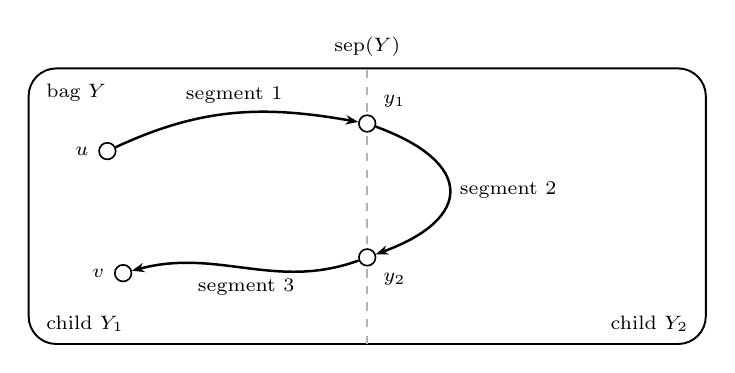
\begin{tikzpicture}[x=1cm,y=1cm]
\draw[line width=0.7pt,rounded corners=10pt] (-4.3,-1.75) rectangle (4.3,1.75);
\node[lab,anchor=north west] at (-4.2,1.68) {bag $Y$};
\draw[faint,dashed,line width=0.7pt] (0,-1.75) -- (0,1.75);
\node[lab,anchor=south] at (0,1.78) {$\mathrm{sep}(Y)$};
\node[lab,anchor=south west] at (-4.2,-1.72) {child $Y_1$};
\node[lab,anchor=south east] at (4.2,-1.72) {child $Y_2$};
\node[v,label={[lab]left:$u$}] (u) at (-3.3,0.7) {};
\node[v,label={[lab]above right:$y_1$}] (y1) at (0,1.05) {};
\node[v,label={[lab]below right:$y_2$}] (y2) at (0,-0.65) {};
\node[v,label={[lab]left:$v$}] (v) at (-3.1,-0.85) {};
\draw[arc,line width=0.9pt] (u) to[out=25,in=170] node[lab,above]{segment $1$} (y1);
\draw[arc,line width=0.9pt] (y1) to[out=-20,in=20,looseness=2.1] node[lab,right]{segment $2$} (y2);
\draw[arc,line width=0.9pt] (y2) to[out=200,in=15] node[lab,below]{segment $3$} (v);
\end{tikzpicture}

\caption{A request $(u,v)$ in a bag $Y$ with two children. The path of least hops in $J$ is $u,y_1,y_2,v$,
and each hop becomes a segment, a request in one child. The intervals of the segments in one child are disjoint, by the \hyperref[lem:A]{Interval Lemma}.}
\label{fig:requests}
\end{figure}

\paragraph{Interior nodes are hubs.} Every $y_i$ with $0<i<k$ is in $\sep^+(Y)$. So, by induction, a start of a request that is
not in $\sep^+$ of the parent is $s$, and an end that is not is $t$. In fact $y_i$ is in $\sep(Y)$: two consecutive
arcs with one label would have a shortcut, so $y_i$ lies on two children.

\paragraph{No communication.} Broadcast $L(s)$ and $L(t)$ over the BFS tree of the root, in $\Ot(D)$ rounds. Then
every vertex $w$ computes the requests of every bag on $w$, top down, with no further messages. If $w$ is on $Y$
then $w$ is on the parent of $Y$, so by induction $w$ knows the requests of the parent. Arcs of $J$ between hubs
are known by (B5). An arc at $s$ with $s$ off $\sep^+(Y)$ comes from $\Out(s,Y_j)\cap\sep^+(Y)$, since
$\sep^+(Y)\subseteq\sep^+(Y_j)$, and an arc at $t$ likewise from $\In(t,Y_j)$. An arc $(s,t)$ comes from
Fact~\ref{fact:query}.

\subsection{Disjointness}

\begin{named}{Interval Lemma}\label{lem:A}
Distinct requests in one bag have disjoint intervals.
\end{named}
\begin{proof}
This holds at the root. Let two segments lie in the child $C$ of $Y$. If they come from different requests $R,R'$
of $Y$, then $\Int(\text{segment};C)\subseteq\Int(R;Y)$: a vertex $x$ with $y_{i-1}\reach_C x\reach_C y_i$ satisfies
$u\reach_Y y_{i-1}\reach_Y x\reach_Y y_i\reach_Y v$, because arcs of $J$ are realized in children of $Y$. So they
are disjoint by induction. If they come from one request, as segments $a<b$, and share $x$, then
$y_{a-1}\reach_C x\reach_C y_b$. Hence $(y_{a-1},y_b)$ is an arc of $J$, which replaces $b-a+1\ge2$ hops by one,
against least hops.
\end{proof}

Only one property of the path is used here: it has no shortcut in $J$. The next lemma uses a little more.
Every request $R$ of $Y$ will get a walk $W(R)$, defined below, that lies in the interval of $R$.

\begin{lemma}[visits]\label{lem:B}
A vertex of $\sep(Y)$ lies on $W(R)$ for at most one request $R$ of $Y$, and has at most two visits in it.
\end{lemma}
\begin{proof}
The intervals of distinct requests are disjoint by the \hyperref[lem:A]{Interval Lemma}. Within $R$, let $x$ lie on segments
$a<b$, and suppose $b\ge a+2$. Either the two are in one child, against the Interval Lemma, or $x$ is in $\sep(Y)$
by (B3), and then $y_{a-1},x,y_b$ is a path in $J$ that replaces $b-a+1\ge3$ hops by two, against least hops. So
$x$ lies on at most two segments, which are consecutive. Each segment path is simple, so this gives at most two
visits.
\end{proof}

\subsection{Realization, bottom up}

Every request $R=(u,v)$ of $Y$ gets a simple directed $uv$-path $\pi(R)$ inside $\Int(R;Y)$. In a leaf this is the
BFS path. Otherwise let $W(R)$ be the concatenation of $\pi$ over the segments of $R$, and let $\pi(R)$ be its
chronological loop erasure: at the first vertex that repeats, jump to its last visit, and continue.

\begin{lemma}[repeats]\label{lem:C}
A vertex that repeats in $W(R)$ lies in $\sep(Y)$.
\end{lemma}
\begin{proof}
Each $\pi(\text{segment})$ is simple. Two segments in one child are disjoint by the \hyperref[lem:A]{Interval Lemma},
as $\pi(\text{segment})$ lies in its interval. Segments in different children meet only on vertices lying on two
children, which are in $\sep(Y)$ by (B3).
\end{proof}

Since $\pi(R)\subseteq W(R)\subseteq\Int(R;Y)$, the paths $\pi$ of distinct requests in $Y$ are disjoint. Consecutive
segments can meet at a hub other than their common end. This happens when a directed cycle runs through two
children and $J$ has a tie, which is why erasure is needed.

\subsection{Doing the erasure}

Fix a request $R$ of a bag. Give an arc of a leaf path that belongs to $W(R)$ its \emph{key}: the sequence of segment
indices along the chain of bags from this bag down to the leaf, followed by the index on the leaf path. Keys are
compared only within one request, since two requests of one bag have keys that look alike. Keys in lexicographic order follow the walk.
A key has $O(\log^2n)$ bits, and every endpoint of the arc knows it with no communication, since it computed the
requests. The key of a visit is the key of the arc leaving it. The end $v$ of a request needs no key since it never
repeats: if $v$ lay on a segment $a<k$, then $(y_{a-1},v)$ would be a shortcut in $J$. The same holds for $u$.

Process levels bottom up. In each bag $Y$, every $x$ in $\sep(Y)$ sends the keys of its retained visits over $T_Y$, and
all vertices of $Y$ compute the same erasure. By Lemma~\ref{lem:B} this is at most $2|\sep(Y)|$ keys, that is,
$\Ot(D)$ words and $\Ot(D)$ rounds. An erased stretch of $R$ is a half-open interval of keys of $R$, from the first
visit up to the last visit, which is kept. Each endpoint of an arc compares the key with the intervals of its own
request. By Lemma~\ref{lem:C} no vertex off $\sep(Y)$ needs to report anything.

\begin{algorithm}[t]
\caption{\AlgPath{}$(s,t)$}\label{alg:path}
\begin{algorithmic}[1]
\State Broadcast the labels $L(s)$ and $L(t)$ over the BFS tree of the root.
\State Every vertex computes, with no messages, the requests of all bags that hold it, top down.
\For{each level, bottom up, all bags of the level in parallel}
  \State Each $x\in\sep(Y)$ sends the keys of its retained visits over $T_Y$.
  \State All vertices of $Y$ compute the same erasure for each request of $Y$.
\EndFor
\State Each vertex outputs its retained arcs.
\end{algorithmic}
\end{algorithm}

\begin{proof}[Proof of the \LemPath{}]
At the root, the retained arcs form $\pi(s,t)$, and each vertex knows its own arcs. The total is $\Ot(D)$ rounds per
level over $O(\log n)$ levels. The statement of~\cite[Lemma 16]{P20} is randomized given a BDD, but its Step 1 as written uses no
randomness. So the algorithm is deterministic relative to the decomposition.
\end{proof}

\section{Bipartite matching}\label{sec:bip}

\subsection{Outer recursion}

Find the bipartition by BFS in $O(D)$ rounds. Compute a BDD of $G$, whose bags we call \emph{outer}. The scheme is the
sequential one of~\cite{LT80}. Process depths bottom up. A leaf solves $G[X^\circ]$ locally, together with an optimal
dual in the weighted case. In an inner bag, by Fact~\ref{fact:depth}, the matchings of the children together are maximum on $G[X^\circ\setminus\sep(X)]$.
Then insert the vertices of $\sep(X)\cap X^\circ$ one at a time, the $i$-th in every bag of the depth during step $i$.

\subsection{One insertion}

Let $M$ be maximum on $G[C]$ with $C\subseteq X^\circ$, and $h$ a new vertex. The maximum size grows by at most $1$, and
if it grows there is an $M$-augmenting path starting at $h$ (compare~\cite[Proposition 1]{IKNS22}, from~\cite{IOO18}).
Indeed, an augmenting path that avoids $h$ would lie in $G[C]$, against maximality. So every augmenting path ends at the free vertex
$h$, and $M\oplus M'$, for a maximum $M'$ on $G[C\cup\{h\}]$, holds at most one. Take the residual digraph on $C\cup\{h\}$,
with arcs leaving the side of $h$ along unmatched edges and returning along matched edges.

\paragraph{The network.} Treat $X$ as its own network, of hop diameter $\Ot(D)$ by (B1). To let edges carry messages without being arcs, subdivide every edge of $X$ once. An
edge in the residual digraph $a\to b$ becomes $a\to w\to b$, and any other edge $a-b$ becomes $a\to w\leftarrow b$,
where $w$ is simulated by an endpoint. All black boxes run with one number of vertices, $4n$, which is at least the size of
this network by planarity: pad it with virtual pendant vertices at one vertex, simulated by it, which keeps planarity. The result is a
planar digraph with the same underlying graph after every flip, whose hop diameter is at most $2\,\mathrm{diam}+O(1)$, and $w$ with two in-arcs is a sink, so paths never use it. Compute one BDD
of this network, an \emph{inner} BDD, once. The inner BDD is separate on purpose: its separators are unrelated to
those of the outer recursion, and a hub of the outer bag can be an interior vertex of an augmenting path.

\begin{algorithm}[t]
\caption{\AlgBip{}, for one bag $X$ and one new vertex $h$}\label{alg:bip}
\begin{algorithmic}[1]
\State Run~\cite[Lemma 16]{P20} on the current digraph, over the inner BDD.
\State Broadcast $L(h)$. Each free vertex $t$ of the other side tests $h\reach t$ by Fact~\ref{fact:query}.
\State Elect one such $t$ over the tree. If there is none, $M$ stays.
\State Otherwise broadcast $L(t)$, run \AlgPath{}$(h,t)$, and flip $M$ along the path.
\end{algorithmic}
\end{algorithm}

A simple path is what makes the flip correct: a walk with a repeated vertex would not leave a matching.
Figure~\ref{fig:insertion} shows one insertion.

\begin{figure}[t]
\centering
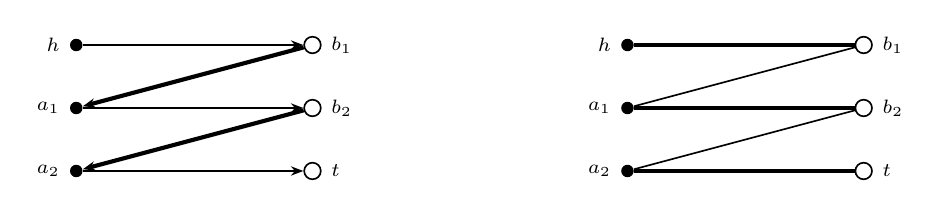
\begin{tikzpicture}[x=1cm,y=1cm]
\foreach \dx/\after in {0/0,7/1}{
\begin{scope}[xshift=\dx cm]
\node[d,label={[lab]left:$h$}] (h) at (0,1.2) {};
\node[d,label={[lab]left:$a_1$}] (a1) at (0,0.4) {};
\node[d,label={[lab]left:$a_2$}] (a2) at (0,-0.4) {};
\node[v,label={[lab]right:$b_1$}] (b1) at (3,1.2) {};
\node[v,label={[lab]right:$b_2$}] (b2) at (3,0.4) {};
\node[v,label={[lab]right:$t$}] (t) at (3,-0.4) {};
\ifnum\after=0
  \draw[arc] (h) -- (b1);
  \draw[arc,line width=1.5pt] (b1) -- (a1);
  \draw[arc] (a1) -- (b2);
  \draw[arc,line width=1.5pt] (b2) -- (a2);
  \draw[arc] (a2) -- (t);
\else
  \draw[e,line width=1.5pt] (h) -- (b1);
  \draw[e] (b1) -- (a1);
  \draw[e,line width=1.5pt] (a1) -- (b2);
  \draw[e] (b2) -- (a2);
  \draw[e,line width=1.5pt] (a2) -- (t);
\fi
\end{scope}}
\end{tikzpicture}

\caption{One insertion. Left: $M$ in thick lines, the new vertex $h$, and the arcs of the residual digraph that $h$
reaches. The vertex $t$ is free and on the other side. Right: $M$ after the flip along the simple path from $h$ to $t$.}
\label{fig:insertion}
\end{figure}

\begin{proof}[Proof of the \ThmBip{}]
Each step of Algorithm~\ref{alg:bip} takes $\Ot(D)$ rounds by (B1) and (B5). There are $\Ot(D)$ steps per depth by (B1), and
$O(\log n)$ depths, so $\Ot(D^2)$ rounds in total. Correctness is the insertion above and induction over the depths.
\end{proof}

\section{Exact labels and weighted matching}\label{sec:weighted}

\subsection{Exact labels}

A \emph{digraph on $G$} has its arcs on edges of $G$, with nonnegative integer lengths of polynomial size, zero allowed.
We write $d_X$ for distances in the part of the digraph inside the bag $X$, and $B(X)=\sep^+(X)\cap V(X)$.

\begin{named}{Exact Labels Lemma}\label{lem:labels}
Given a BDD, in $\Ot(D^2)$ rounds, for every bag $X$, every vertex $v$ of $X$ and every $a\in B(X)$, the vertex $v$
learns $d_X(a,v)$ and $d_X(v,a)$. This is deterministic relative to the decomposition.
\end{named}
\begin{proof}
We have $|B(X)|=\Ot(D)$ by (B1), since the tree has height $O(\log n)$. If $Y$ is a child of $X$, then
$B(X)\cap V(Y)\subseteq B(Y)$, since $\sep^+(X)\subseteq\sep^+(Y)$.

Induct from the leaves. A leaf has $\Ot(D)$ vertices by (B4), and so $\Ot(D)$ arcs by planarity. It broadcasts them over a BFS
tree of the leaf in $\Ot(D)$ rounds, and each vertex computes the distances.

Let $X$ be an inner bag with children $Y_1,\dots,Y_k$, and assume the claim for the children. Let $Q$ be the digraph on
$B(X)$ with an arc from $a$ to $b$ of length $\min_jd_{Y_j}(a,b)$, over the children that hold both. Each $a$ in $B(X)$
knows these values for its children, and it lies on at most three of them, by (B3). It broadcasts them over $T_X$. That is
$\Ot(D^2)$ words in all, so $\Ot(D^2)$ rounds, for all bags of a depth in parallel by (B2). Each vertex of $X$ now knows $Q$
and computes all-pairs distances $d_Q$.

We have $d_Q=d_X$ on $B(X)$. An arc of $Q$ is a walk in a child, which is a subgraph of $X$, so $d_X\le d_Q$. Conversely,
cut a shortest path of $X$ from $a$ to $b$ at its vertices in $B(X)$. Each piece has no inner vertex on $\sep(X)$, since
$\sep(X)\subseteq B(X)$. So by Fact~\ref{fact:cut} it lies in one child, and its length is at least that of the arc of $Q$.

For $v$ in $V(X)$ and $a$ in $B(X)$,
\[
d_X(a,v)=\min_{Y\ni v,\ b\in B(X)\cap V(Y)}\bigl(d_Q(a,b)+d_Y(b,v)\bigr),
\]
with $d_X(a,v)=d_Q(a,v)$ if $v$ is in $B(X)$, and symmetrically for $d_X(v,a)$. The value on the right is the length of a walk in
$X$. For the other direction, take a shortest path from $a$ to $v$ and let $b$ be its last vertex in $B(X)$. If $b=v$ we are
done. Otherwise the rest has no inner vertex on $\sep(X)$, and neither is $v$ on it, so by Fact~\ref{fact:cut} this rest lies in
the one child that holds $v$. So the formula attains $d_X(a,v)$. The vertex $v$ knows $d_Y(b,v)$ by induction and $d_Q$ from the
broadcast, so this needs no further messages. There are $O(\log n)$ depths.
\end{proof}

\begin{named}{Offset Theorem}\label{thm:off}
After the \LemLabels{}, for any offsets $\varphi(u)$, each a nonnegative integer of polynomial size or $\infty$ and known to its
own vertex, every vertex $v$ learns $\min_u(\varphi(u)+d_G(u,v))$ in $\Ot(D)$ further rounds.
\end{named}
\begin{proof}
For a bag $X$ and a hub $h\in\sep(X)$ let
\begin{align*}
A_X(h)&=\min_{u:\,X\text{ on the chain of }u}\bigl(\varphi(u)+d_X(u,h)\bigr),\\
d(v)&=\min_{X\text{ on the chain of }v}\ \min_{h\in\sep(X)}\bigl(A_X(h)+d_X(h,v)\bigr).
\end{align*}
This is the Virtual Source Lemma of~\cite{S26} with $\varepsilon=0$. We recall the argument. Each term is the length of
a walk, so $d(v)$ is at least the true value. Conversely, take a best $u$ and a shortest path $P$ to $v$, and descend from the root
as long as $P$ avoids the separator. By Fact~\ref{fact:cut} the path stays in one child, which is on the chains of $u$ and of $v$,
and by (B4) it must meet a separator, at a hub $h$ of a bag $X$ that holds all of $P$. The terms for $X$ and $h$ then give the length of $P$.

Each bag has $\Ot(D)$ values $A_X(h)$. One pipelined convergecast and one broadcast over $T_X$ take $\Ot(D)$ rounds, for
all bags of a depth in parallel, and there are $O(\log n)$ depths.
\end{proof}

With positive lengths, each vertex takes a tight in-arc, which gives a shortest-path forest. Zero lengths go away
by $\ell'=(n+1)\ell+1$ and $\varphi'=(n+1)\varphi$, with $d=\lfloor d'/(n+1)\rfloor$.

\subsection{Weighted matching}

Keep integers $y$ on the current set $C$ with the following, where edges, sides and free vertices are those of $G[C]$,
and of $G[C\cup\{h\}]$ during the insertion of $h$:
\begin{enumerate}[(D1)]
\item $y\ge0$ and $y(a)+y(b)\ge w(ab)$ for every edge,
\item $y(a)+y(b)=w(ab)$ on $M$,
\item $y(v)=0$ on free $v$.
\end{enumerate}
Then $M$ is optimal: any matching $N$ has $w(N)\le\sum_{uv\in N}(y(u)+y(v))\le\sum y(v)=w(M)$.

\paragraph{Insertion of $h$.} Say $h$ is in $A$; the case of $B$ is symmetric. Set
$y(h):=\max(0,\max_{b\sim h}(w(hb)-y(b)))$, which restores (D1). Use the arcs $a\to b$ on unmatched edges with length
$y(a)+y(b)-w(ab)\ge0$, and $b\to a$ on matched edges with length $0$. Let $d$ be the distance from $h$, and set
\[
\delta=\min\bigl(\min_{\text{free }b}d(b),\ \min_{a\in A}(d(a)+y(a))\bigr).
\]
The term $a=h$ gives $\delta\le y(h)$. Let $z$ attain the minimum. Update
\[
y'(a)=y(a)-\max(0,\delta-d(a)),\qquad y'(b)=y(b)+\max(0,\delta-d(b)).
\]
\begin{itemize}
\item We have $y'(a)\ge0$, since $\delta\le d(a)+y(a)$. For a free $b$, $y'(b)=0$, since $\delta\le d(b)$.
\item Unmatched edge: if $d(a)\ge\delta$ nothing decreases. Otherwise $d(b)\le d(a)+\ell$ gives
$y'(a)+y'(b)\ge y(a)+y(b)-\ell=w(ab)$.
\item Matched edge: $a\ne h$ has only the in-arc from its partner, so $d(a)=d(b)$, and the sum is unchanged.
\item An arc on a shortest path with $d(b)\le\delta$ becomes tight. Every vertex on a shortest path to $z$ has $d\le d(z)\le\delta$.
\end{itemize}
Flip along a simple shortest path from $h$ to $z$. If $z=h$, then $\delta=y(h)$, so $y'(h)=0$ and $h$ stays free. If $z=b$ is free, then
$y'(z)=0$ and $z$ becomes matched, which is allowed in any case. If $z=a\ne h$, then $y'(a)=0$ and $a$ becomes free, as (D3) requires.
All of (D1) to (D3) hold on $C\cup\{h\}$, and integers stay integers.

\paragraph{Distributed.} By (D1) to (D3), $y\le\max w$, also for $y(h)$, so all lengths are at most $2\max w$ and fit in
$O(1)$ words. A vertex that $h$ does not reach has $d=\infty$, and the \LemLabels{} and the \ThmOff{} allow this.

\begin{algorithm}[t]
\caption{\AlgWeight{}, for one bag $X$ and one new vertex $h$}\label{alg:weight}
\begin{algorithmic}[1]
\State Compute labels by the \LemLabels{} over the inner BDD, and $d$ by the \ThmOff{} with $\varphi(h)=0$.
\State Elect $\delta$ and $z$ by aggregation on the tree of $X$, and update $y$ locally.
\State Each edge sees whether it is tight under $y'$, so the tight arcs form a planar digraph.
\State Run \AlgPath{}$(h,z)$ on the tight arcs, over the subdivided network, and flip $M$.
\end{algorithmic}
\end{algorithm}

In the digraph of tight arcs under $y'$, any $hz$-path has length $d(z)$, so \AlgPath{} gives a simple shortest
path, and no parent pointers are used.

\begin{proof}[Proof of the \ThmWeight{}]
An insertion takes $\Ot(D^2)$ rounds, by the \LemLabels{} and the \ThmOff{}. There are $\Ot(D)$ insertions per depth and
$O(\log n)$ depths. For a perfect matching, replace $w$ by $Kn-w$ with $K$ above every weight. A maximum weight matching then has
maximum cardinality, and among those, minimum original weight.
\end{proof}

\section{Many sources and vertex covers}\label{sec:ms}

\begin{proof}[Proof of the \LemMS{}]
For every bag $Y$ let $R(Y)$ be the union of $\Out(a,Y)\cap\sep(Y)$ over the sources $a$ in $Y^\circ$. A vertex $a$ in $Y^\circ$
has $Y$ on its chain, so it knows this set from its label. Since $R(Y)\subseteq\sep(Y)$, an OR over $T_Y$ gives it to all of $Y$
in $\Ot(D)$ rounds per level. A vertex $v$ answers yes if $v$ is a source, or if $\In(v,Y)\cap R(Y)\ne\emptyset$ for some $Y$ on
its chain.

A yes is sound, with $\In$ and $\Out$ reflexive. Conversely let $P$ be a path from a source $a$ to $v$. Descend from the root as long as
$P$ avoids the separator. By Fact~\ref{fact:cut} it stays in one child, so it meets the separator of a bag $Y$ whose proper
ancestors it avoided. Hence $a$ and $v$ are in $Y^\circ$, and the vertex met is in $\Out(a,Y)\cap\In(v,Y)$.
\end{proof}

\begin{proof}[Proof of Corollary~\ref{cor:konig}]
Given $M$, let $Z$ be the set reached from free vertices of $A$ in the residual digraph. As usual, $(A\setminus Z)\cup(B\cap Z)$ is
a vertex cover of size $|M|$, and its complement is a maximum independent set. The \LemMS{}, run on the subdivided network of
Section~\ref{sec:bip}, gives $Z$ in $\Ot(D)$ rounds.
\end{proof}

\section{General planar networks}\label{sec:general}

The method carries sequential work over to CONGEST. Maximum matchings of planar graphs by nested dissection are given in~\cite{MS06},
and elimination with pivoting on matrices of low treewidth in~\cite{FLPSW18}. Lemma~\ref{lem:mate} is from~\cite{RV89}, the principal
submatrix below is~\cite[Theorem 5.6]{FLPSW18}, and the update of Lemma~\ref{lem:update} is in~\cite[Theorem 7, Section 4.3]{MS06}. The
check with odd components goes back to~\cite{Kar86}, and the check of Section~\ref{sec:cert} is the one
of~\cite[Section 3.1, Theorem 3.4]{Che97}, with one random kernel vector in place of a kernel basis. What is new here is the distributed
form: the elimination moves $\Ot(D^2)$ words per bag, a singular interior block is handled by keeping at most $|\partial X|$ further
indices, mates are found with few solves per hub, and the check runs on the bags in $\Ot(D)$ rounds.


Here words are field elements of a prime field $\F_p$, $p=n^{O(1)}$. Let $k=\max_X|\sep^+(X)|=\Ot(D)$. By (B3), for a non-leaf $X$,
\begin{equation}\label{eq:sumpartial}
\sum_{Y\text{ child of }X}|\partial Y|\le|\partial X\setminus\sep(X)|+3|\sep(X)|\le3|\sep^+(X)|\le3k.
\end{equation}
By Fact~\ref{fact:edge} we assign each edge to the deeper home of its ends, and let $O_X$ be the set of edges assigned to $X$. All edges at a vertex
$x$ with home $Z$ lie in $O_Y$ for bags $Y$ in the subtree of $Z$. The graph $G$ is simple, so a planar graph on $\sep^+(X)$ has at most $3k$ edges, and
$|O_X|\le3k$. Each end learns the home of the other end in $\Ot(1)$ rounds, so it knows $O_X$. Let $c_X$ be the root of $T_X$.

\subsection{Elimination in the tree of bags}

Let $A$ be an alternating matrix over $\F_p$ on an index set $W\subseteq V$, with entries only on edges of $G$. Write $A_e$ for the part of an edge $e$. A matrix $M$ is \emph{alternating} if $M^T=-M$ and its diagonal is zero. \emph{Eliminating} a nonsingular principal block on $P$ means passing to $M_{Q,Q}-M_{Q,P}M_{P,P}^{-1}M_{P,Q}$ on the remaining indices $Q$, and this keeps a matrix alternating. An alternating
matrix of rank $r$ has a nonsingular principal submatrix of size $r$, on any row basis.

\begin{lemma}[one step]\label{lem:onestep}
Let $M$ be alternating on the disjoint union of $I$ and $\partial$. Choose $P\subseteq I$ with $M_{P,P}$ nonsingular and $|P|=\rank M_{I,I}$. Let
$M'$ be the result of eliminating $P$, on $(I\setminus P)\cup\partial$. Choose $I''\subseteq I\setminus P$ such that the rows of
$M'_{I\setminus P,\partial}$ indexed by $I''$ are a basis of its row space. Then $M'_{I\setminus P,I\setminus P}=0$, $|I''|\le|\partial|$, and with $M''$
the restriction of $M'$ to $I''\cup\partial$,
\[
\rank M=|P|+\rank M''.
\]
\end{lemma}
\begin{proof}
The rank adds over an elimination, inside the block on $I$ too, so the block of $M'$ on $I\setminus P$ has rank $0$. So a row of $M'$ with index
$d\in I\setminus P\setminus I''$ is zero on $I\setminus P$, and on $\partial$ it is a combination of the rows of $I''$, which are zero on $I\setminus P$ as well.
So row $d$ is a combination of rows of $I''$ in $M'$, and by alternation the same holds for columns. Deleting $d$ keeps the rank.
\end{proof}

Figure~\ref{fig:step} shows the step. It bounds the size of what a bag passes to its parent by the size of its boundary,
whatever the rank of the interior.

\begin{figure}[t]
\centering
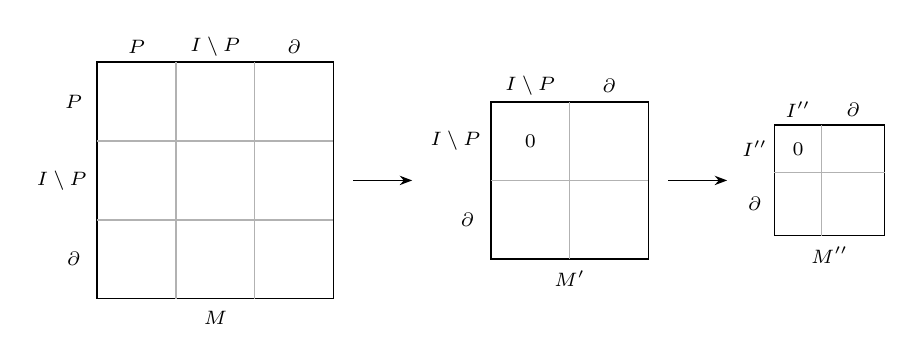
\begin{tikzpicture}[x=1cm,y=1cm]
% M
\draw[line width=0.6pt] (0,0) rectangle (3,3);
\draw[faint] (1,0) -- (1,3) (2,0) -- (2,3) (0,1) -- (3,1) (0,2) -- (3,2);
\node[lab] at (-0.3,2.5) {$P$};
\node[lab] at (-0.45,1.5) {$I\setminus P$};
\node[lab] at (-0.3,0.5) {$\partial$};
\node[lab] at (0.5,3.2) {$P$};
\node[lab] at (1.5,3.2) {$I\setminus P$};
\node[lab] at (2.5,3.2) {$\partial$};
\node[lab] at (1.5,-0.25) {$M$};
\draw[arc] (3.25,1.5) -- (4.0,1.5);
% M'
\begin{scope}[xshift=5 cm,yshift=0.5 cm]
\draw[line width=0.6pt] (0,0) rectangle (2,2);
\draw[faint] (1,0) -- (1,2) (0,1) -- (2,1);
\node[lab] at (-0.45,1.5) {$I\setminus P$};
\node[lab] at (-0.3,0.5) {$\partial$};
\node[lab] at (0.5,2.2) {$I\setminus P$};
\node[lab] at (1.5,2.2) {$\partial$};
\node[lab] at (0.5,1.5) {$0$};
\node[lab] at (1,-0.25) {$M'$};
\end{scope}
\draw[arc] (7.25,1.5) -- (8.0,1.5);
% M''
\begin{scope}[xshift=8.6 cm,yshift=0.8 cm]
\draw[line width=0.6pt] (0,0) rectangle (1.4,1.4);
\draw[faint] (0.6,0) -- (0.6,1.4) (0,0.8) -- (1.4,0.8);
\node[lab] at (-0.25,1.1) {$I''$};
\node[lab] at (-0.25,0.4) {$\partial$};
\node[lab] at (0.3,1.6) {$I''$};
\node[lab] at (1,1.6) {$\partial$};
\node[lab] at (0.3,1.1) {$0$};
\node[lab] at (0.7,-0.25) {$M''$};
\end{scope}
\end{tikzpicture}

\caption{Lemma~\ref{lem:onestep}. Left: $M$ with the pivots $P$, the rest $I\setminus P$ of the interior and the boundary
$\partial$. Middle: after the elimination, $M'$ has a zero block on $I\setminus P$. Right: a bag passes on only $M''$, on the
retained rows $I''$, at most $|\partial|$ of them, and on $\partial$.}
\label{fig:step}
\end{figure}

\begin{algorithm}[t]
\caption{\AlgElim{}$(W)$}\label{alg:elim}
\begin{algorithmic}[1]
\For{each bag $X$, bottom up, all bags of a depth in parallel}
  \State Form $M_X=\sum_{Y\text{ child of }X}M''_Y+\sum_{e\in O_X}A_e$, restricted to $W$, on an index set $J_X\subseteq V(X)$ that also holds
  the vertices of $W$ with home $X$. Let $I_X=J_X\setminus\partial X$.
  \State Apply Lemma~\ref{lem:onestep} with $I=I_X$ and $\partial=J_X\cap\partial X$. This gives $P_X$, $I''_X$, the dropped set
  $D_X=I_X\setminus(P_X\cup I''_X)$, and $M''_X$ on $I''_X\cup(J_X\cap\partial X)$.
\EndFor
\end{algorithmic}
\end{algorithm}

All of this is local at $c_X$. The set $P_X$ can be found by $2\times2$ pivots: take the next $i\in I_X$, take $j\in I_X$ with nonzero entry, if any, and
eliminate $\{i,j\}$. A row with no such $j$ stays zero on $I_X$ in later steps.

\begin{lemma}[correctness]\label{lem:elimcorrect}
Every vertex of $W$ is in exactly one $P_X$ or one $D_X$. Let $B=\bigcup P_X$ and $N=\bigcup D_X$. Then $\rank A=|B|$, and $A_{B,B}$ is nonsingular.
\end{lemma}
\begin{proof}
Let $N_t$ be the sum of all $M''_Y$ of processed bags whose parent is not processed yet, and of all $A_e$ with $e$ assigned to unprocessed bags, so
$N_0=A$. By Fact~\ref{fact:edge}, the row of an index $x\in I_X$ in $N_t$ lies inside $M_X$: $x$ has its home in the subtree of $X$, its edges are assigned in that
subtree, and by (B3) $x$ lies in no sibling. Indices of $M''_Y$ are in $V(Y)$, so a retained index stays in one bag per depth. So Lemma~\ref{lem:onestep},
applied to $N_t$ with $I=I_X$ and everything else as $\partial$, gives $\rank N_t=|P_X|+\rank N_{t+1}$, since the rows in $I_X$ are zero outside $J_X$. At the
root $\partial$ is empty, so $I''_{\mathrm{root}}=\emptyset$ and $N_{\mathrm{final}}=0$. So $\rank A=\sum|P_X|$.

Now run the same steps on $A_{B,B}$ with the same pivots. Eliminations on indices in $B$ use only pivots in $B$ and entries in $B$, so each matrix of
that run is the restriction of the matrix above to $B$, and every index is pivoted in the end. Hence $\det A_{B,B}=\prod_X\det(M_X)_{P_X,P_X}\ne0$.
\end{proof}

\begin{lemma}[rounds]\label{lem:elimrounds}
The elimination takes $\Ot(D^2)$ rounds. Afterwards $c_X$ holds the pivot rows of $X$, and each vertex knows whether it is in $B$.
\end{lemma}
\begin{proof}
A vertex $v\in V(X)$ knows from its chain whether $v\in\partial X$. So an upcast over $T_X$ gives $c_X$ the set $\partial X$, in $\Ot(D)$ words. By
Lemma~\ref{lem:onestep}, the index set of $M''_Y$ has at most $2|\partial Y|$ elements, so $M''_Y$ has at most $4|\partial Y|^2$ entries. By~\eqref{eq:sumpartial} the
matrices of the children of $X$ have at most $4(3k)^2=\Ot(D^2)$ entries in total. The vertex $c_Y$ lies in $V(Y)\subseteq V(X)$, and sends them over $T_X$. The
set $O_X$ adds at most $3k$ words. So bags of one depth do this in parallel in $\Ot(D^2)$ rounds, and there are $O(\log n)$ depths. The sets $P_X$ and
$D_X$, of at most $\Ot(D)$ words since $|I_X|\le\sum_Y|\partial Y|+|\sep(X)|$, go back over $T_X$.
\end{proof}

A leaf is the same with $\sep(X)=V(X)$: $c_X$ receives its $\Ot(D)$ edges.

\paragraph{Solving.} Let $A_{W,W}$ be nonsingular, so $N=\emptyset$ by Lemma~\ref{lem:elimcorrect}. Given $b$ with $b_v$ known at $v$, solve $A_{W,W}x=b$ as follows.
Upward: $y_X$ on $J_X$ is the sum of $y''_Y$ over children and of $b_v$ for the vertices with home $X$; $c_X$ applies the pivots,
$y'_q=y_q-M_{q,P}M_{P,P}^{-1}y_P$, and passes $y''_X$ on $I''_X\cup(J_X\cap\partial X)$ to its parent. Downward: given $x$ on that set from the parent, $c_X$
computes $x_P=M_{P,P}^{-1}(y_P-M_{P,\mathrm{rest}}x_{\mathrm{rest}})$, broadcasts $x_P$ over $T_X$, and sends each child its part. By~\eqref{eq:sumpartial} each depth
moves $\Ot(D)$ words. So one system takes $\Ot(D)$ rounds, and every vertex learns $x_v$.

\begin{named}{Linear Algebra Lemma}\label{lem:la}
Let a matrix over $\F_p$, $p=n^{O(1)}$, be symmetric or alternating, and have nonzero entries only on the diagonal and on edges of $G$, with each entry known to
its row and column vertices. In $\Ot(D^2)$ rounds the network computes its rank, a set $B$ of size equal to the rank with nonsingular principal submatrix, and
a factorization stored at the vertices $c_X$, after which each system on $B$ is solved in $\Ot(D)$ rounds, every vertex learning its coordinate.
\end{named}
\begin{proof}
For alternating matrices this is what we have shown: if $N$ is not empty, a second run of the elimination on $W=B$, within the same bound, has $N=\emptyset$, since
$A_{B,B}$ is nonsingular. For symmetric matrices the steps are the same with $1\times1$ and $2\times2$ pivots, since a symmetric matrix of rank $r$ also has a
nonsingular principal submatrix of size $r$ on any row basis. A diagonal entry is added at the home of its vertex.
\end{proof}

\subsection{Mates}

Let $p$ be the least prime at least $n^3$, found after one aggregation of $n$. For each edge $e=uv$ with $u<v$, the vertex $u$ draws $a_e$ uniformly in $\F_p^\times$, and $A$ is
the matrix with $A_{uv}=a_e$, $A_{vu}=-a_e$, and zero elsewhere.

\begin{fact}[\cite{RV89}]\label{fact:tutte}
Always $\rank A\le2\nu(G)$, and $\rank A=2\nu(G)$ with probability at least $1-n/p$.
\end{fact}
Indeed, $\det A_{W,W}$ is the square of a polynomial in the $a_e$ with one term for each perfect matching of $G[W]$. So if $A_{W,W}$ is nonsingular, then $G[W]$ has a perfect matching. Conversely, for the vertex set $W$ of a
maximum matching, this is a nonzero polynomial of degree $\nu(G)$, and it vanishes with probability at most $\nu(G)/(p-1)$.

Run the elimination on $W=V$. By Lemma~\ref{lem:elimcorrect}, $G[B]$ has a perfect matching, and $|B|=\rank A$. It remains to find one. Bags run top down by depth, and all
bags of one depth in parallel and in lock step, with phases of fixed length.

\begin{lemma}[mate]\label{lem:mate}
Let $A_{W,W}$ be nonsingular with inverse $F$, and $s\in W$. Then there is $v\in W$ with $A_{s,v}\ne0$ and $F_{v,s}\ne0$. For every $v\ne s$, the matrix $A$ on
$W\setminus\{s,v\}$ is nonsingular if and only if $F_{v,s}\ne0$.
\end{lemma}
\begin{proof}
From $(AF)_{s,s}=1=\sum_vA_{s,v}F_{v,s}$ we get the first claim. The identity on complementary minors of a matrix and its inverse gives $\det A_{W\setminus T,W\setminus T}=\det A_{W,W}\cdot\det F_{T,T}$,
and for $T=\{s,v\}$ the alternating $F$ gives $\det F_{T,T}=F_{s,v}^2$.
\end{proof}

\begin{lemma}[update]\label{lem:update}
Let $R\subseteq W$ with $F_{R,R}$ nonsingular, and $W'=W\setminus R$. Then $A_{W',W'}$ is nonsingular, with inverse $F_{W',W'}-F_{W',R}(F_{R,R})^{-1}F_{R,W'}$.
\end{lemma}
\begin{proof}
The identity on complementary minors gives nonsingularity, and the block formula for an inverse gives the rest.
\end{proof}

\begin{algorithm}[t]
\caption{\AlgMates{}, search at a bag $X$; $W_X$ is the set of unmatched vertices of $B$ in $X^\circ$}\label{alg:mates}
\begin{algorithmic}[1]
\State Run \AlgElim{}$(W_X)$ on the subtree of $X$. Let $R=\emptyset$, and let $F$ be the inverse of $A$ on $W_X$.
\For{each hub $s\in\sep(X)\cap W_X$ in order of identifiers, unless $s$ is already matched}
  \State $c_X$ announces $s$ over $T_X$; neighbours exchange whether they lie in $W_X\setminus R$.
  \State Solve for the column $F_{\cdot,s}$. Each $r\in R$ sends $F_{r,s}$ to $c_X$, which computes $w=(F_{R,R})^{-1}F_{R,s}$ and broadcasts it.
  \State Each $v\in W_X\setminus R$ computes $g(v)=F_{v,s}-\sum_{r\in R}F_{v,r}w_r$. Each neighbour $v$ of $s$ tells $s$ whether $g(v)\ne0$.
  \State The hub $s$ takes the neighbour $v$ with $g(v)\ne0$ of least identifier, and announces it.
  \State Solve for the column $F_{\cdot,v}$. Each $r\in R\cup\{s\}$ sends $F_{r,v}$ to $c_X$. Let $R\leftarrow R\cup\{s,v\}$.
\EndFor
\end{algorithmic}
\end{algorithm}

By Lemma~\ref{lem:update}, $g(v)$ is the entry $(v,s)$ of the inverse on $W_X\setminus R$. At a leaf, all vertices of $W_X$ are hubs. In the first step, $W_X\cap\partial X=\emptyset$, so the run ends at $X$ with nothing left, and by
Lemma~\ref{lem:elimcorrect} and nonsingularity no vertex is dropped.

\begin{lemma}[search]\label{lem:search}
The search needs no random choice to succeed: if $A_{B,B}$ is nonsingular, as Lemma~\ref{lem:elimcorrect} states, then every hub finds a mate, and at the end the vertices of $B$
are perfectly matched. All of it takes $\Ot(D^2)$ rounds.
\end{lemma}
\begin{proof}
By Lemmas~\ref{lem:mate} and~\ref{lem:update}, $A$ stays nonsingular on $W_X\setminus R$, and $F_{R,R}$ stays nonsingular, since the same identity relates it to that minor. After the
search at $X$, all hubs are matched, so for a non-leaf the remaining vertices lie in children of $X$ by (B3). At depth $\ell$, let $W$ be all unmatched vertices of $B$. Their homes have
depth at least $\ell$, so each lies in $X^\circ$ for one bag $X$ of depth $\ell$. By Fact~\ref{fact:depth} no edge joins $W_X$ and $W_{X'}$ for $X\ne X'$, so $A_{W,W}$ is the block diagonal of the
$A_{W_X,W_X}$, and each block is nonsingular. So the hypothesis holds at the next depth. Every vertex of $B$ is matched when its home is reached.

Rounds at one depth: the elimination takes $\Ot(D^2)$ by Lemma~\ref{lem:elimrounds}. There are at most $\Ot(D)$ hubs, each with two solves in $\Ot(D)$ rounds and with $|R|\le2|\sep(X)|$
words to and from $c_X$, so $\Ot(D^2)$ in total, for all bags of the depth in parallel. There are $O(\log n)$ depths.
\end{proof}

\begin{proof}[Proof of the \ThmGen{}]
By construction $M$ is a perfect matching of $G[B]$, so a matching of size $|B|/2=\rank(A)/2\le\nu(G)$ by Lemma~\ref{lem:elimcorrect} and Fact~\ref{fact:tutte}, and equal to $\nu(G)$ with probability at
least $1-n/p$.
\end{proof}

\subsection{The certificate}\label{sec:cert}

Let $N=V\setminus B$. Each $d\in N$ draws $z_d$ uniformly in $\F_p$. Set $y_N=z$, and $y_B=-(A_{B,B})^{-1}A_{B,N}z$, which is one system with $b_v=-\sum_{d\in N}A_{v,d}z_d$, known to $v$ after one
round, on the second run of the elimination with $W=B$. Let $D'=\{v:y_v\ne0\}$, $A'=N(D')\setminus D'$, and $C'$ the rest.

\begin{lemma}[kernel]\label{lem:kernel}
We have $Ay=0$, and $z\mapsto y$ is a bijection onto the kernel of $A$. For $v$ in the union $Z$ of the supports of kernel vectors, $y_v\ne0$ with probability at least $1-1/p$.
\end{lemma}
\begin{proof}
The rows on $B$ vanish by construction. Rows on $B$ are a basis of the row space by Lemma~\ref{lem:elimcorrect}, so the rows on $N$ vanish too. The dimension of the kernel is $|N|$, and $y_N=z$, so the
map is onto. For $v\in Z$, $y_v$ is a nonzero linear form in $z$.
\end{proof}

\begin{lemma}[missed vertices]\label{lem:missed}
With probability at least $1-O(n^2/p)$, $D'=D(G)$, where $D(G)$ is the set of vertices missed by some maximum matching.
\end{lemma}
\begin{proof}
Assume $\rank A=2\nu(G)$ and $\rank A_{-v,-v}=2\nu(G-v)$ for all $v$; by Fact~\ref{fact:tutte} this fails with probability at most $(n+1)n/p$. If $v\in Z$, say $Au=0$ with $u_v\ne0$, then also $u^TA=0$, so
row $v$ is a combination of other rows, and column $v$ as well. So $\rank A_{-v,-v}=\rank A$, that is $\nu(G-v)=\nu(G)$, and $v\in D(G)$. Conversely, if $\nu(G-v)=\nu(G)$, take a row basis of $A$ avoiding $v$, of
size $\rank A_{-v,-v}=\rank A$; then row $v$ is a combination of it, which gives a kernel vector with nonzero entry at $v$. So $Z=D(G)$, and Lemma~\ref{lem:kernel} with a union bound gives the claim.
\end{proof}

\paragraph{Odd components.} For any set $S$, the number $\odd(G-S)$ of odd components can be counted without error in $\Ot(D)$ rounds. Bottom up, a bag $X$ holds the partition of $\partial X\setminus S$ induced by the graph of the
subtree, with parity per block, and a count of closed odd blocks. The vertex $c_X$ merges the partitions of the children and the edges of $O_X$, and adds $1$ to the parity of each vertex off $S$ with home $X$. A block with no
vertex of $\partial X$ is closed. Each vertex is counted once, each edge once, and by Fact~\ref{fact:edge} a closed block has no further edge. By~\eqref{eq:sumpartial}, each depth moves $\Ot(D)$ words.

\begin{proof}[Proof of the \ThmCert{}]
The check has two parts: (a) $n-2|M|=\odd(G-A')-|A'|$, and (b) $\odd(G-A'-D')=0$. Each is one run of the count above.

\emph{A pass is correct, with no assumption on the randomness.} For any $S$, the deficiency formula~\cite{LoP86} gives $n-2\nu(G)\ge\odd(G-S)-|S|$, so by (a) $M$ is maximum, and $A'$ attains the bound. So
$\rank A=|B|=2|M|=2\nu(G)$. If $v\in D'$, then $Ay=0$ and $y^TA=0$ with $y_v\ne0$ give $\rank A_{-v,-v}=\rank A$, and $\rank A_{-v,-v}\le2\nu(G-v)$ by Fact~\ref{fact:tutte}, so $v\in D(G)$. Conversely, since $A'$
attains the bound, every maximum matching misses only vertices of odd components of $G-A'$. No edge joins $D'$ to $C'$, by the definition of $A'$, so each component of $G-A'$ lies in $D'$ or in $C'$, and by (b) the odd ones lie
in $D'$. So $D(G)\subseteq D'$. Hence $D'=D(G)$, $A'=N(D(G))\setminus D(G)=A(G)$ and $C'=C(G)$.

\emph{A correct run passes.} If $D'=D(G)$ and $|M|=\nu(G)$, both parts hold by the structure theorem of~\cite{LoP86}: $A'=A(G)$, the components of $G[D(G)]$ are odd and factor-critical, and those of $C(G)$ are even, with
$n-2\nu(G)=c(D(G))-|A(G)|$. By Lemma~\ref{lem:missed} and Fact~\ref{fact:tutte}, a run passes with probability at least $1-O(n^2/p)=1-O(1/n)$, and repeating $O(1)$ times gives high probability with $\Ot(D^2)$ rounds.
\end{proof}

Part (b) cannot be left out. On the path $a$-$b$-$c$ with $z_d=0$ we get $D'=A'=\emptyset$, and (a) holds, while $D(G)=\{a,c\}$.

\section{Treewidth \texorpdfstring{$\tau$}{tau}}\label{sec:tw}

Here $G$ need not be planar, and we replace the BDD by the decomposition of~\cite{IKNS22}.
\begin{enumerate}[(T1)]
\item \cite[Theorem 1 and Lemma 13]{IKNS22}. In $\Ot(\tau^2D+\tau^3)$ rounds, with high probability, we get a rooted tree of depth $O(\log n)$. A node $x$ has a connected subgraph $G_x$, the part $G'_x=G_x-B_{p(x)}$, connected too, and
$S_x\subseteq V(G'_x)$, called $S'_x$ in~\cite{IKNS22}. The bag is $B_x=(V(G_x)\cap B_{p(x)})\cup S_x$, of size $O(t)$ for $t=O(\tau^2\log n)$. The children of $x$ are the components of $G'_x-S_x$, each with its edges to $B_x$. A non-leaf has $|S_x|=O(\tau^2)$. At a leaf,
$S_x=V(G'_x)$, of size $O(t)$. Each vertex knows its bags. The doubling of~\cite{IKNS22} leaves every vertex with an estimate of $\tau$ of at most $2(\tau+1)$. One aggregation makes it common, so phases below can have fixed lengths.
\item \cite[Lemma 9, Theorem 6, Corollary 3]{IKNS22}. On the $G_x$ of one depth, $h$ sums take $\Ot(\tau D+h\tau)$ rounds with high probability, by the dilation $\Ot(\tau D)$ and congestion $h\Ot(\tau)$ of~\cite[Lemma 9]{IKNS22} and the scheduling
of~\cite[Theorem 6]{IKNS22}, and $h$ broadcasts take the same by~\cite[Corollary 3]{IKNS22}. These are stated for a near disjoint collection,~\cite[App.~A.1]{IKNS22}. Its first condition speaks of all edges of $G$, and it can fail here: two adjacent
vertices of a bag can both lie in the graphs of two children. The proof of~\cite[Lemma 7]{IKNS22} uses it only for edges inside a subgraph, and that form holds. Each edge of $G_C$ has an end in $G'_C$, which lies in no other subgraph of that
depth, $G'_C$ is connected, and each other vertex of $G_C$ has an edge into $G'_C$.
\end{enumerate}

The home of $v$ is the first $x$ with $v\in S_x$. Fact~\ref{fact:edge} holds: the proof of~\cite[Lemma 13]{IKNS22} shows that the homes of an edge are comparable, and that the end with the shallower home lies in the bag of the deeper one. So edges are
assigned as before, and the two ends of an edge of $O_x$ lie in $B_x$, with one end in $G'_x$. Section~\ref{sec:general} holds with $\partial x=V(G_x)\cap B_{p(x)}$, except for the rounds, since~\eqref{eq:sumpartial} fails: a bag can have many children,
each with up to $t$ boundary vertices and $t$ retained rows. Two changes repair this.

\paragraph{Sums per entry.} First $t$ broadcasts make $B_x$ and $B_x\cap W$ known in $G_x$, so that sums have a common index. Children only add on boundary indices. For $u,w\in B_x$ the entry of $M_x$ is the sum of $M''_C[u,w]$ over children $C$, plus
the entry of an edge of $O_x$. One vertex of $G'_C$, its least identifier, inputs each value of $C$. So $t^2$ sums suffice, whatever the number of children.

\paragraph{A filter for retained rows.} Let $U$ be the union of the sets $I''_C$. Rows of $U$ are zero on $U$: inside one child by Lemma~\ref{lem:onestep}, and between two children since their interior indices share no entry. So each row of $U$ is a vector on
$B_x$, of $t$ words, and any row in the span of other rows of $U$ can be dropped, by the argument of Lemma~\ref{lem:onestep}. To find a basis $U_0$, repeat at most $t+1$ times: the holder of each row tests it against the span of the rows broadcast so far, one
aggregation finds the least identifier outside the span, and its holder broadcasts its $t$ words. This costs $\Ot(\tau D+t\tau)$ per iteration. So $|U_0|\le t$. The index set is $J_x=U_0\cup(B_x\cap W)$.

Then every vertex of $G_x$ knows $M_x$ on $J_x$, and all of them apply Lemma~\ref{lem:onestep} with the same deterministic rule. So every vertex of $G_x$ knows $P_x$, $I''_x$ and $M''_x$. This is what the holders use at the parent. Each depth costs
\[
t\cdot\Ot(\tau D+t\tau)+\Ot(\tau D+t^2\tau)=\Ot(\tau^3D+\tau^5).
\]

\paragraph{Solving.} A system on a nonsingular block drops nothing, so $U_0=U$ there, and $|U|\le t$. The vector $y$ on $B_x$ is $t$ sums, and $y$ on $U$ is $t$ broadcasts. Downward no broadcast is needed: $G_x\subseteq G_{p(x)}$, so each vertex of $G_x$ knows the solution on
$J_{p(x)}$ and computes it on $P_x$ itself. So each depth costs $\Ot(\tau D+\tau^3)$.

\paragraph{Mates.} The search has at most $|S_x|=O(\tau^2)$ hubs per inner bag, and at most $t=O(\tau^2\log n)$ in a leaf, where every vertex is a hub. Each uses two solves and $\Ot(t)$ broadcasts, and each vertex of $G_x$ then knows $F_{R,R}$ and $F_{R,s}$, so it
computes $w$ itself. A neighbour reports over its own edge. By Fact~\ref{fact:edge}, the $G'_x$ are vertex disjoint at one depth and their active vertices are not joined, so Lemma~\ref{lem:search} holds. Each depth costs $\Ot(\tau^3D+\tau^5)$.

\paragraph{Certificate.} One solve gives $D'$ and $A'$. The components of $G-A'$ follow from~\cite[Lemma 8]{IKNS22}, and one aggregation per component gives its parity, in $\Ot(\tau D)$ rounds. A component lies in $D'$ or in $C'$, so the same run gives both parts of the check.

\begin{proof}[Proof of the \ThmTw{}]
Sum over $O(\log n)$ depths. Fact~\ref{fact:tutte} and Lemma~\ref{lem:missed} hold on any graph, and a pass of the check is correct as in Section~\ref{sec:cert}. What remains random is (T1) and (T2), which hold with high probability, so we do not claim zero error here. The bound $\Ot(\tau^3D+\tau^5)$ also covers the $\Ot(\tau^2D+\tau^3)$ of (T1).
\end{proof}

The width $t=O(\tau^2\log n)$ of (T1) is what costs: a decomposition of width $\Ot(\tau)$ in the same rounds would give $\Ot(\tau^2D+\tau^3)$.

\section{Proof of Corollary~\ref{cor:paths}}\label{sec:cors}

\paragraph{Vertex cover.} Let $G$ be bipartite with sides $L$ and $L'$, and take $D',A',C'$ of Section~\ref{sec:cert}. If these are the canonical sets, then $A'\cup(L\cap C')$ is a vertex cover of size $\nu(G)$. Components of $G[D(G)]$ are factor-critical
and bipartite, so single vertices. So $D(G)$ is independent with neighbours in $A(G)$, and an edge inside $C(G)$ has an end in $L$. Further $n-2\nu=|D|-|A|$ gives $\nu=|A|+|C|/2$, and $C(G)$ has a perfect matching, so $|L\cap C|=|C|/2$. Each vertex decides
locally. A failed cover check is detected by one aggregation.

\paragraph{Disjoint paths.} Let $V'=V\setminus\{s,t\}$. Let $\kappa_0$ be the maximum number of paths that have at least one inner vertex, so $\kappa=\kappa_0+1$ if $s\to t$ is an arc and $\kappa=\kappa_0$ if not. Each $v\in V'$ hosts the vertices $v^-$, $v^+$, and
$a_v$ if $s\to v$ is an arc, and $z_v$ if $v\to t$ is an arc. Let $H$ have the edges $v^+v^-$ for each $v$, $a_vv^-$, $v^+z_v$, and $u^+v^-$ for each arc $u\to v$ in $V'$. A vertex $x$ of $G$, in a bag or a separator, stands for all its hosted vertices, so each
bag at most quadruples and the proofs above apply, with $p$ chosen for $|V(H)|\le4n$: edges of $H$ are local or lie on one edge of $G$. Then $\nu(H)=|V'|+\kappa_0$. Indeed the self edges $v^+v^-$ are a matching, and a path $v_1,\dots,v_\ell$ from $N^+(s)$ to
$N^-(t)$, with $\ell\ge1$, replaces $\ell$ self edges by $\ell+1$ edges.

Conversely, let $M$ be a maximum matching of $H$. Its edges $u^+v^-$ form vertex disjoint paths and cycles on $V'$, where a vertex $v$ on none of them counts as a path of one vertex unless $M$ has its self edge. Measured against the self edges, a path gains
$1$ if it uses $a$ at its start and $z$ at its end, gains $0$ if it uses one of them, and loses $1$ if it uses neither, which a maximum matching excludes. So exactly $\kappa_0$ paths use both. The vertices of one path learn which kind it is by one aggregation over a
vertex disjoint family of connected subgraphs: $\Ot(\tau D)$ by~\cite[Lemma 8]{IKNS22}, and $\Ot(D)$ on planar networks by the bags, with an upward pass as for odd components and a downward pass that hands the result of each closed block to its vertices. The
other paths and the cycles are ignored.

\paragraph{The separator.} If there is no arc from $s$ to $t$, then $\kappa=\kappa_0$. Take the cover $C$ of the previous paragraph on $H$, so $|C|=|V'|+\kappa$. For $v\in V'$ the self edge puts $v^+$ or $v^-$ in $C$. Let $S$ be the set of those $v$ for which $C$ contains both
of them, or $a_v$, or $z_v$. Each such $v$ has an extra copy in $C$, so $|S|\le\kappa$. The set $S$ separates $s$ from $t$. Indeed, take a path $s,v_1,\dots,v_\ell,t$ avoiding $S$. Since $a_{v_1}\notin C$, the edge $a_{v_1}v_1^-$ gives $v_1^-\in C$, so $v_1^+\notin C$. The
edge $v_i^+v_{i+1}^-$ then gives $v_{i+1}^-\in C$ and $v_{i+1}^+\notin C$. So $v_\ell^+\notin C$ and $z_{v_\ell}\notin C$, and the edge $v_\ell^+z_{v_\ell}$ is not covered, a contradiction. By the duality of disjoint paths and separators~\cite{LoP86}, $|S|=\kappa$. Each vertex decides locally from its copies.

\section{Numerical checks}\label{sec:numerics}

The scripts are in the directory \texttt{sim/} of the repository named in Section~\ref{sec:lean}. They run the logic centrally on decompositions in which every edge lies in a child and a vertex off the separator lies in
exactly one child. Their separators are two paths of a BFS tree or come from the region bags of~\cite{S26}. Nothing enforces the
size, height or balance of (B1) and (B4), an option puts a whole separator on every child, against (B3), and leaves are forced on region bags. Every planar instance is checked for planarity with \texttt{networkx}. No proof uses these checks. Table~\ref{tab:num} lists the main lanes. Timed lanes do not reproduce exact counts on another machine.

\begin{table}[t]
\centering\small
\begin{tabular}{@{}p{5.4cm}rp{7.6cm}@{}}
\toprule
Lane & Runs & Compared with\\
\midrule
Path Lemma, \texttt{run.py path} & 807,500 & simple, right ends, every step an arc\\
Matching, weights, vertex cover, \texttt{run.py} & 55,503 & independent matching and weighted solvers, brute force\\
General, \texttt{gm.py} & 61,752 & rank of the whole matrix, independent blossom algorithm, brute-force $D(G)$\\
General on region bags, \texttt{gm.py region} & 17,209 & the same, up to $n=542$\\
Treewidth, \texttt{gm.py tw} & 52,455 & the same, up to $n=126$\\
Tiny primes, \texttt{gm.py tiny} & 35,553 & each of 25,205 passes of the check right against brute force\\
Disjoint paths, \texttt{gm.py paths} & 12,510 & independent maximum flow, reachability test for the separator\\
Exact labels, \texttt{labels.py} & 26,521 & an independent shortest-path solver: 558,792,578 labels and 3,897,456 queries, up to $n=348$\\
\bottomrule
\end{tabular}
\caption{Main lanes. No check failed in any of them.}
\label{tab:num}
\end{table}

Negative controls are deliberately wrong rules that have to fail. Any path in $J$ in place of least hops gives overlapping intervals and non-simple paths. Without the erasure, the path lane gives $57$ non-simple paths in $6{,}250$ runs, while the matching lane does not fire, since residual
digraphs there rarely produce a repeat ($312$ in $55{,}503$ runs). So the erasure is tested by the path lane. A wrong $\delta$ and stopping at the first free vertex give wrong weights. In the general lanes, a mate that is any edge, no correction after pivots, no retained rows, no elimination step and a field of
size $3$ or $5$ all fire, and at tiny primes part (a) of the check alone passed a wrong $D'$ on $6{,}440$ runs, while the full check never passed a wrong answer. Words per bag grow as $D^2$ on grids, with words$/D^2$ between $3.1$ and $7.4$ up to $n=900$. The controls of the labels lane are the rule with $\sep$ in place of $\sep^+$, no all-pairs step on $Q$, and queries at the deepest bag or at the root only. All of them fire.

The limits are these. There is no CONGEST simulation, so rounds are not measured. The black boxes of~\cite{P20} and the real bags of~\cite{LP19} are not implemented. Sizes stop at about $225$ vertices in the path and matching lanes, $348$ in the general and labels lanes, $542$ on region bags and $126$ in the treewidth lane, and six single grids up to $900$ measure words. Separators in the treewidth lane are chosen by degree, so neither their size nor their
balance is that of~\cite{IKNS22}. The symmetric case of the \LemLA{} is not run.

\section{Formal verification}\label{sec:lean}

The formalization is in the directory \texttt{lean/PlanarMatching/} of the repository
\begin{center}
\url{https://github.com/ssenge/ExactPlanarBipartiteMatching}.
\end{center}
It uses Lean~4 with the toolchain \texttt{leanprover/lean4:v4.36.0-rc1} and Mathlib at the revision
\begin{center}
\texttt{d875a8de5222f62cf1c2fafc7984588adadc990a},
\end{center}
which is pinned in \texttt{lean/lake-manifest.json}. No proof uses \texttt{sorry}. The file \texttt{lean/axioms.txt} records the axioms of all theorems named below, and it lists only \texttt{propext}, \texttt{Classical.choice} and \texttt{Quot.sound}. In a fresh clone, run
\texttt{lake exe cache get} first. These files prove the following from abstract hypotheses:
\begin{itemize}
\item \texttt{LoopErase}: the erasure of a walk is simple, keeps both ends and its arcs, and reports from the set of repeated vertices suffice.
\item \texttt{Requests}: least hops gives no shortcut, the \hyperref[lem:A]{Interval Lemma} and Lemma~\ref{lem:C} for two different segments (\texttt{lemmaC}).
\item \texttt{Decomp}: from (B2), (B3), (B4) and the inclusion of a child in its parent, the form of Fact~\ref{fact:cut} in which a whole interval avoids the separator (\texttt{stays}) and its form for a walk whose inner vertices avoid the separator (\texttt{walk\_stays}), Fact~\ref{fact:query}, the core of the \LemMS{} (\texttt{descent}, \texttt{multiSource}), a walk in $J$ (\texttt{jpath}), and the claims of Fact~\ref{fact:depth} (\texttt{chain\_comparable}, \texttt{arc\_in\_chain}, \texttt{no\_cross}), and the distance formula of the \LemLabels{}, with distances as least walk lengths and the hub digraph $Q$, under the hypothesis that the children cover the bag (\texttt{exact\_labels}, \texttt{distQ\_eq}, in \texttt{Labels}).
\item \texttt{Hungarian}: weak duality, the dual update, the flip along a simple alternating path, and their combination \texttt{insertion}.
\item \texttt{Tutte}: over any field, Lemma~\ref{lem:onestep} (\texttt{one\_step}), Lemma~\ref{lem:mate} (\texttt{mate\_exists}, \texttt{jacobi\_block}, \texttt{alternating\_two\_minor}, \texttt{minor\_ne\_zero\_iff}), Lemma~\ref{lem:update} (\texttt{update\_inverse}), the steps these use, that the inverse of an alternating matrix is alternating (\texttt{IsAlternating.inv}), and the deficiency bound for any matching and any set (\texttt{tutte\_berge\_weak}).
\end{itemize}
Not in Lean, among others: planarity, Fact~\ref{fact:edge}, Lemma~\ref{lem:B}, the \LemPath{} as a whole, the facts taken from~\cite{LP19,P20,IKNS22}, anything about rounds or knowledge, the growth by at most $1$ in one insertion, that distances satisfy the stated inequalities, the correspondence from a simple path in the residual digraph to the list used by \texttt{flip}, the induction of Lemma~\ref{lem:elimcorrect} over bags, Fact~\ref{fact:tutte}, Lemmas~\ref{lem:search}, \ref{lem:kernel} and~\ref{lem:missed}, the step that uses the structure theorem, Section~\ref{sec:tw}, the rounds of the \LemLabels{} and the \ThmOff{}.

\section{Open questions}\label{sec:open}

\begin{itemize}
\item Matching in $\Ot(D)$ rounds. In the bipartite case, batching hubs that lie on a face, since paths in a planar digraph cannot cross without meeting, is the natural attempt, but augmentations interact. In the general case, a dense matrix on a boundary of size $D$ has $\Theta(D^2)$ words, so a faster bound needs another compression.
\item Maximum weight matching in $\Ot(D^2)$ rounds with no hypothesis, and for general planar networks. The algebraic route has polynomials of degree $nW$ in the weight variable, and it was noted in~\cite{FLPSW18} that its approach does not extend easily to weights.
\item Whether the \ThmGen{} can be made deterministic. Apart from the decomposition it uses randomness only in the $a_e$, and the \ThmCert{} also in the $z_d$.
\item A decomposition of width $\Ot(\tau)$ in the rounds of (T1), which would give $\Ot(\tau^2D+\tau^3)$ in the \ThmTw{}.
\end{itemize}

\section*{Use of AI}

The proofs, the code and the Lean files were developed with Claude Opus~5.5 (Anthropic), which was also used to search the literature and to draft the text. They were reviewed by separate AI referees, by adversarial AI agents that searched for counterexamples, and by the numerical
scripts of Section~\ref{sec:numerics}.

\begin{thebibliography}{99}
\bibitem{ADW26a} Y.~Abd-Elhaleem, M.~Dory, O.~Weimann. A Simple Distributed Deterministic Planar Separator. SIROCCO 2026, arXiv:2602.22916.
\bibitem{ADPW25} Y.~Abd-Elhaleem, M.~Dory, M.~Parter, O.~Weimann. Distributed Maximum Flow in Planar Graphs. PODC 2025, arXiv:2411.11718.
\bibitem{AKO18} M.~Ahmadi, F.~Kuhn, R.~Oshman. Distributed Approximate Maximum Matching in the CONGEST Model. DISC 2018.
\bibitem{Che97} J.~Cheriyan. Randomized $\tilde O(M(|V|))$ algorithms for problems in matching theory. SIAM J.\ Comput.\ 26(6), 1635--1655, 1997.
\bibitem{dV23} T.~de~Vos. Minimum Cost Flow in the CONGEST Model. SIROCCO 2023, arXiv:2304.01600.
\bibitem{FHLRS25} N.~Fischer, B.~Haeupler, R.~Latypov, A.~Roeyskoe, A.~L.~Sulser. A Simple Parallel Algorithm with Near-Linear Work for Negative-Weight Single-Source Shortest Paths. SOSA 2025, 216--225, arXiv:2410.20959.
\bibitem{FLPSW18} F.~V.~Fomin, D.~Lokshtanov, M.~Pilipczuk, S.~Saurabh, M.~Wrochna. Fully polynomial-time parameterized computations for graphs and matrices of low treewidth. ACM Trans.\ Algorithms, 2018, arXiv:1511.01379.
\bibitem{GH16} M.~Ghaffari, B.~Haeupler. Distributed Algorithms for Planar Networks I: Planar Embedding. PODC 2016.
\bibitem{IOO18} Y.~Iwata, T.~Ogasawara, N.~Ohsaka. On the Power of Tree-Depth for Fully Polynomial FPT Algorithms. STACS 2018.
\bibitem{IKNS22} T.~Izumi, N.~Kitamura, T.~Naruse, G.~Schwartzman. Fully Polynomial-Time Distributed Computation in Low-Treewidth Graphs. SPAA 2022, arXiv:2205.14897.
\bibitem{IKY23} T.~Izumi, N.~Kitamura, Y.~Yamaguchi. A Nearly Linear-Time Distributed Algorithm for Exact Maximum Matching. SODA 2024, arXiv:2311.04140.
\bibitem{JMR25} B.~Jauregui, P.~Montealegre, I.~Rapaport. Deterministic Distributed DFS and Other Problems via Cycle Separators in Planar Graphs. PODC 2025, arXiv:2504.21620.
\bibitem{Kar86} H.~Karloff. A Las Vegas RNC algorithm for maximum matching. Combinatorica 6(4), 387--391, 1986.
\bibitem{KI21} N.~Kitamura, T.~Izumi. A Subquadratic-Time Distributed Algorithm for Exact Maximum Matching. IEICE Trans.\ Inf.\ Syst.\ E105-D(3), 2022, arXiv:2104.12057.
\bibitem{LoP86} L.~Lov\'asz, M.~D.~Plummer. Matching Theory. Annals of Discrete Mathematics 29, North-Holland, 1986.
\bibitem{LP19} J.~Li, M.~Parter. Planar Diameter via Metric Compression. STOC 2019.
\bibitem{LTY26} H.~Le, H.~Tierno, S.~Yang. Planar Embedding of Okamura-Seymour Quasimetrics in Polynomial Time with an Application to Distributed SSSP. arXiv:2606.31192.
\bibitem{LT80} R.~J.~Lipton, R.~E.~Tarjan. Applications of a planar separator theorem. SIAM J.\ Comput.\ 9(3), 1980.
\bibitem{MN95} G.~L.~Miller, J.~Naor. Flow in planar graphs with multiple sources and sinks. SIAM J.\ Comput.\ 24(5), 1995.
\bibitem{MS06} M.~Mucha, P.~Sankowski. Maximum Matchings in Planar Graphs via Gaussian Elimination. Algorithmica 45, 2006.
\bibitem{P20} M.~Parter. Distributed Planar Reachability in Nearly Optimal Time. DISC 2020.
\bibitem{RV89} M.~O.~Rabin, V.~V.~Vazirani. Maximum matchings in general graphs through randomization. Journal of Algorithms 10(4), 557--567, 1989.
\bibitem{S26} S.~Senge. Exact Shortest Paths and Maximum Flow in Planar Networks in the CONGEST Model. Repository \url{https://github.com/ssenge/ExactShortestPathsAndFlowsOnPlanarGraphs}.
\end{thebibliography}

\end{document}
